\documentclass{article}
\usepackage[paperwidth=15cm,paperheight=8.5cm,margin=4mm]{geometry}
\usepackage{amsmath}
\usepackage{tikz}
\usetikzlibrary{arrows.meta,positioning,fit,backgrounds}
\pagestyle{empty}

% Figure Contract
% Core claim: one mechanism links inputs to outcomes and is supported by two distinct checks.
% Evidence: replace all placeholders with traced model/results artifacts.
% Reader path: inputs -> central Hero -> outcomes; then inspect support Panels.
% Hero: central mechanism, largest and uniquely accented.
% Supporting evidence: upper Panel explains assumptions; lower Panel verifies behavior.
% Removable items: remove any Panel that repeats the Hero rather than adding evidence.

\begin{document}\noindent
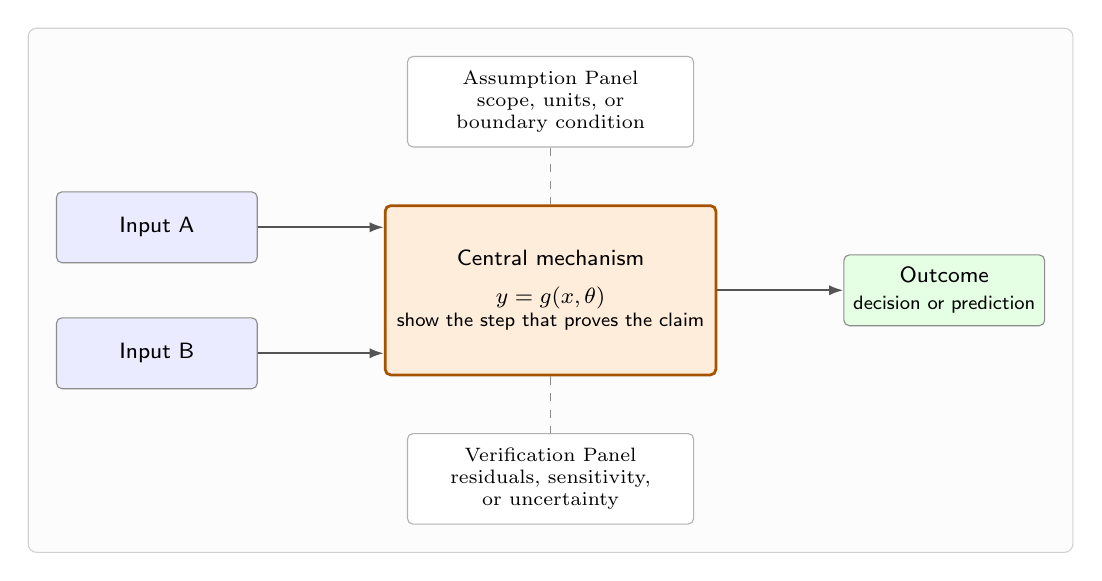
\begin{tikzpicture}[
  font=\sffamily\footnotesize,
  block/.style={draw=black!45, fill=black!3, rounded corners=2pt,
    minimum width=2.55cm, minimum height=0.9cm, align=center},
  panel/.style={draw=black!30, fill=white, rounded corners=2pt,
    text width=3.4cm, minimum height=1.15cm, align=center, font=\scriptsize},
  flow/.style={-{Latex[length=1.8mm,width=1.3mm]}, line width=0.75pt, draw=black!67}
]
  \node[block, fill=blue!8] (sourceA) at (0,0.8) {Input A};
  \node[block, fill=blue!8] (sourceB) at (0,-0.8) {Input B};
  \node[block, fill=orange!14, draw=orange!65!black, line width=1.0pt,
    minimum width=4.2cm, minimum height=2.15cm] (hero) at (5.0,0)
    {Central mechanism\\[4pt]$y=g(x,\theta)$\\[-1pt]
     \scriptsize show the step that proves the claim};
  \node[block, fill=green!10] (outcome) at (10.0,0) {Outcome\\\scriptsize decision or prediction};
  \draw[flow] (sourceA.east) -- (hero.west |- sourceA.east);
  \draw[flow] (sourceB.east) -- (hero.west |- sourceB.east);
  \draw[flow] (hero) -- (outcome);

  \node[panel, above=0.72cm of hero] (assumptionPanel)
    {Assumption Panel\\\scriptsize scope, units, or boundary condition};
  \node[panel, below=0.72cm of hero] (verificationPanel)
    {Verification Panel\\\scriptsize residuals, sensitivity,\\or uncertainty};
  \draw[black!45, dashed] (assumptionPanel) -- (hero);
  \draw[black!45, dashed] (hero) -- (verificationPanel);

  \begin{scope}[on background layer]
    \node[fit=(sourceA)(sourceB)(outcome)(assumptionPanel)(verificationPanel),
      inner sep=10pt, fill=black!1, draw=black!18, rounded corners=3pt] {};
  \end{scope}
\end{tikzpicture}
\end{document}
